\section{Simulation of the \texorpdfstring{$\mathrm{e}^{+} \mathrm{e}^{-} \to \mathrm{q} \bar{\mathrm{q}}$}{ee -> qqbar} scattering process at fixed-order QED}

For the first part of this project, a Monte Carlo integrator was developed to evaluate the cross-section for the process $\mathrm{e}^{-} \mathrm{e}^{+} \to \mathrm{q} \bar{\mathrm{q}}$ to leading-order. In this section, after a brief introduction to the relevant properties of the differential cross-section to be integrated, the general idea for the Monte Carlo integrator here developed is discussed. Then, some results for the values of the cross-section and their associated error estimates are presented. Finally, as an example of more advanced implementations of Monte Carlo integrators, the \texttt{vegas} package is used to integrate the differential cross-section, for which the results and its algorithm are commented on.

\subsection{The differential cross-section at leading order}

At leading order, the matrix element for the process $\mathrm{e}^{-} \mathrm{e}^{+} \to \mathrm{q} \bar{\mathrm{q}}$ consists of two $s$-channel contributions which differ by having either a photon or a Z boson as the “intermediary” particle, as shown in the Feynman diagram in \autoref{fig:feynman-diagram}.
\begin{figure}[ht!]
    \centering
    \feynmandiagram [horizontal=a to b] {i1 [particle=\(\mathrm{e}^{+}\)] -- [anti fermion] a -- [anti fermion] i2 [particle=\(\mathrm{e}^{-}\)], a -- [photon, edge label={\(\gamma\), $\mathrm{Z}$}] b, f1 [particle=\(\bar{\mathrm{q}}\)] -- [fermion] b -- [fermion] f2 [particle=\(\mathrm{q}\)], };
    \caption{An $s$-channel process mediated by either a photon or a Z boson.}
    \label{fig:feynman-diagram}
\end{figure} \\
The resulting squared matrix element is then given by
\begin{align}
    &
    \begin{aligned}
    \lvert \mathcal{M}_{\mathrm{q} \bar{\mathrm{q}}} \rvert^{2} = (4 \pi \alpha)^{2} N_{C} & \left[
    \left( 1 + \cos^{2}{\theta} \right) \left\{ Q_{\mathrm{e}}^{2} Q_{\mathrm{q}}^{2} + 2 Q_{\mathrm{e}} Q_{\mathrm{q}} V_{\mathrm{e}} V_{\mathrm{q}} \chi_{1}(s) + \left( A_{\mathrm{e}}^{2} + V_{\mathrm{e}}^{2} \right) \left( A_{\mathrm{q}}^{2} + V_{\mathrm{q}}^{2} \right) \chi_{2}(s) \right\}
    \right. \\
    & \left. \qquad + \cos{\theta} \hspace{2mm} \left\{ 4 Q_{\mathrm{e}} Q_{\mathrm{q}} A_{\mathrm{e}} A_{\mathrm{q}} \chi_{1}(s) + 8 A_{\mathrm{e}} V_{\mathrm{e}} A_{\mathrm{q}} V_{\mathrm{q}} \chi_{2}(s) \right\} \right];
    \end{aligned} \label{eq:1-sqr-mat-element} \\
    & \hspace{3mm} \chi_{1}(s) = \kappa \frac{s(s - M_{\text{Z}}^{2})}{(s - M_{\text{Z}}^{2})^{2} + \Gamma^{2}_{\text{Z}} M_{\text{Z}}^{2}}, \qquad \chi_{2}(s) = \kappa^{2} \frac{s^{2}}{(s - M_{\text{Z}}^{2})^{2} + \Gamma^{2}_{\text{Z}} M_{\text{Z}}^{2}}; \label{eq:1-chi-funcs}
\end{align}
and depends on three kinematic phase-space quantities: 
\begin{enumerate}[label=\roman*)]
    \item $s$, the squared total energy in the centre-of-mass;

    \item $\cos{\theta}$, the cosine of the scattering angle $\theta$ between the incoming positron and the outgoing quark, and

    \item $\phi$, the azimuthal angle of the outgoing quark in the plane perpendicular to the beam.
\end{enumerate}
The meaning and values of the constants in expressions \eqref{eq:1-sqr-mat-element} and \eqref{eq:1-chi-funcs} above are not relevant for the moment but they are given in \autoref{sec:app-num-values}. Instead, the following properties are important:
\begin{itemize}
    \item There is no dependence on $\phi$.
    
    \item The dependence on $\cos{\theta}$ comes only in two forms, $(1 + \cos^{2}{\theta})$ and $\cos{\theta}$. When integrating over $-1 < \cos{\theta} < 1$, the former term yields $8/3$ while the latter is zero. Thus, the interesting part is the dependence on $s$.

    \item The dependence on $s$ comes in two forms (besides the trivial one), given by $\chi_{1}(s)$ and $\chi_{2}(s)$.
\end{itemize}

Finally, the differential cross-section to be integrated is
\begin{equation}\label{eq:1-diff-sigma}
    \frac{\mathrm{d}\sigma}{\mathrm{d}s \, \mathrm{d}(\cos{\theta}) \, \mathrm{d}\phi} = \frac{f_{\text{conv}}}{64 \pi^{2}} \frac{f(s)}{s} \sum_{\mathrm{q} = 1}^{N_{\mathrm{q}}} \lvert \mathcal{M}_{\mathrm{q}\bar{\mathrm{q}}}(s, \cos{\theta}, \phi) \rvert^{2}
\end{equation}
where $f(s)$ is a normalized distribution that defines the beam spectrum, $N_{q}$ is the number of light quark flavours that can be produced, and $f_{\text{conv}}$ is a conversion factor to give the cross-section in picobarns. Therefore, the task of this part will be to integrate \eqref{eq:1-diff-sigma} via Monte Carlo integration and, in the process, apply importance sampling for $s$ as a technique for reducing the variance of the estimated value.

\subsection{Monte Carlo integration with importance sampling}

At a basic level, a Monte Carlo integrator is composed of two ingredients: an integrand and distributions to sample the integration variables. While the integrand for the problem at hand is given by \eqref{eq:1-diff-sigma}, there are three distributions that require to be set: two distributions for the kinematic variables, $s$ and $\cos{\theta}$ (a distribution for $\phi$ is unnecessary, since there is no dependence on it), and the beam distribution $f(s)$. The last one is determined by the specifics of the beam, but the first two require some special consideration, as being able to properly sample the integration space will determine how big the sample size needs to be to compute the integral with a certain accuracy.

A naive first approach could be to sample each variable according to a uniform distribution along its integration interval, a method known as \textit{uniform sampling}. Although easy to implement, this method has the disadvantage of requiring a possibly too large sample size to compute the integrand to a decent accuracy, as it samples regions with small and large contributions to the integral equally. An improvement over this method, could be to allow for specific distributions that attempt to sample regions of the integrand according to their contribution (or importance) to the integral. This method is referred to as \textit{importance sampling}, and it contains uniform sampling as a special case. \emph{For this reason, the integrator here developed was written from the beginning as an importance sampling integrator.}

Importance sampling consists of the following: having an integrand $f(\mathbf{x})$ and a distribution $g(\mathbf{x})$ for the integration variables, $N$ points $\mathbf{x}$ are sampled from $g(\mathbf{x})$, and the estimate of the integral is given by
\begin{equation}
    E_{N} = \frac{1}{N} \sum_{i = 1}^{N} \frac{f(\mathbf{x}_{i})}{g(\mathbf{x}_{i})}.
\end{equation}
The estimated error for the Monte Carlo result is then given by
\begin{equation}
    \lvert \delta E_{N} \rvert = \sqrt{\frac{1}{N} \sum_{i = 1}^{N} \left( \frac{f(\mathbf{x}_{i})}{g(\mathbf{x}_{i})}\right)^{2} - E_{N}^{2}}
\end{equation}
and decreases with sampling size as $1/\sqrt{N}$ as long as the sequence of variances for different $N$ is bounded.

\newpage

Thus, the formulas above establish the sampling method but, alas, one still needs to specify the distribution $g(\mathbf{x})$. As discussed earlier, the most interesting part of the integrand is the dependence on $s$, so for the remainder of this project, the distribution for $\cos{\theta}$ was set to a uniform distribution between $-1$ and $+1$ (excluding the latter), and different distributions for $s$ were chosen, to exemplify the effects of sampling the integrand on the estimation of the integral and its error estimate.

\subsubsection*{Comments on the implementation}
\addcontentsline{toc}{subsubsection}{\protect\numberline{}Comments on the implementation}

The Monte Carlo integrator developed was written in Python3.10 (but compatibility was checked for 3.8 and 3.9 as well) as the \texttt{integrator} module of the python package \texttt{simulator} (great names, right?). The main components for the integrator consist of the following:
\begin{enumerate}
    \item Particle (pseudo-data) classes \texttt{Electron}, \texttt{LightQuarks} and \texttt{ZBoson}, containing the relevant properties of these particles such as charge, weak isospin, etc. These could all have been written as child classes of a parent class \texttt{Particle}. Hindsight is 20/20 and time is running out. 
    
    \item A function defining the squared matrix element in \eqref{eq:1-sqr-mat-element}. It takes as input values for $s$, $\cos{\theta}$ and quark flavour q. For $s$ and $\cos{\theta}$ one can pass either single values, single value and array or two arrays of equal length, whereas for q one can pass a single value or an array of equal length to $s$ and $\cos{\theta}$.

    \item A parent class \texttt{Distribution}, defined by the methods \texttt{sample} and \texttt{evaluate\_distro}, together with three child classes of it: \texttt{Dirac}, \texttt{Uniform} and \texttt{BreitWigner}. The idea is that the Monte Carlo integrator requires only the two methods in the parent class, so one can define any distribution as a child of \texttt{Distribution} and therefore avoid having to modify the integrator to accommodate for other distributions. Additionally, to ensure reproducibility, each \texttt{Distribution} child class should allow the setting of a random number generator if necessary, so upon passing the distributions to the Monte Carlo integrator the generation of random numbers is tied to the integrator instead of independently for each distribution.

    \item A \texttt{MonteCarloIntegrator} class, which can be instanced by passing distributions for $s$, $\cos{\theta}$, $f(s)$ (and even $\phi$ just for the sake of it) and specifying a method to sum over light quark flavours (at the moment the only options are “explicit” and “random”). All of these are optional, defaulting to $f(s) = \delta(s - M_{\mathrm{Z}}^{2})$, uniform distributions for $\cos{\theta}$ and $\phi$, and explicitly summing over all quark flavours. Each instance has a default seed number (integer) which can be modified through the keyword \texttt{seed}. The squared matrix element is hard-coded within the integrator so that's the only thing it can integrate.
    
\end{enumerate}
All the code, data and figures, as well as a few examples on how to instantiate the integrator and compute the cross-section, are available at the GitHub repository \url{https://github.com/VictorG20/mc-particle-physics}.

\newpage

\subsection{Results}

The total cross-section for the squared matrix element in \eqref{eq:1-sqr-mat-element} was computed with the Monte Carlo integrator for the following 3 scenarios, which differ on the sampling methods used for $s$ and the choice of beam distribution $f(s)$:
\begin{enumerate}
    \item Fixed beam energy: $f(s) = \delta(s - M_{\mathrm{Z}}^{2})$, where $M_{\mathrm{Z}}$ is the mass of the Z boson;

    \item Flat beam spectrum and flat $s$ sampling: $f(s)$ is a uniform distribution between $s_{\text{min}} = (M_{\text{Z}} - 3 \Gamma_{\text{Z}})^{2}$ and $s_{\text{max}} = (M_{\text{Z}} + 3 \Gamma_{\text{Z}})^{2}$ and, similarly, $s$ is drawn from such uniform distribution;

    \item Flat beam spectrum and Breit-Wigner importance sampling for $s$: $f(s)$ is the same as in the previous point but now importance sampling is used for $s$, using a Breit-Wigner distribution
    \begin{equation}\label{eq:1-breit-wigner}
        g(s) = \frac{M_{\text{Z}} \Gamma_{\text{Z}}}{\rho(s_{\text{max}}) - \rho(s_{\text{min}})} \frac{1}{(s - M_{\text{Z}}^{2})^{2} + M^{2}_{\text{Z}} \Gamma^{2}_{\text{Z}}}, \qquad \rho(s) = \arctan{ \left( \frac{s - M_{\text{Z}}^{2}}{M_{\text{Z}} \Gamma_{\text{Z}}}\right)}.
    \end{equation}
\end{enumerate}
Furthermore, the sum over quark flavours in \eqref{eq:1-diff-sigma} has been done in two ways: (i) “explicit”, meaning that the sum is carried out as implied in the equation, and (ii) “random”, consisting on picking a random flavour q for each Monte Carlo point and taking $\sum_{\mathrm{q}} \lvert \mathcal{M} \rvert^{2} = N_{f} \langle \lvert \mathcal{M} \rvert^{2} \rangle_{\mathrm{q}}$.

The results for the cross-section for each of the configurations described and both methods of summing over quark flavours are given in \autoref{tab:1-cross-sections}, together with the exact values obtained from solving the integrals analytically. \marginpar{Part b) \\ Answer 1.}Comparing the columns for both methods of evaluating the quark sum, it is clear that \emph{both methods are statistically equivalent: their values and estimated errors yield intersecting intervals.} The importance of this equivalence lies in the possibility of avoiding the explicit sum in favour of the random method for the purpose of computing the cross-section, as the former requires to compute the squared matrix element for each quark flavour. Additionally, as will be discussed in the next section, it allows to classify events with a specific quark flavor for processes such as showering.

\begin{table}[ht!]
    \centering
    \renewcommand{\arraystretch}{1.5}
    \begin{tabular}{|c|c|c|c|c|}
        \hline \multicolumn{2}{|c|}{} & \multicolumn{3}{c|}{Cross-section (pb)} \\ \hline
        $s$ distribution & $f(s)$ & Explicit quark sum & Random quark flavour & Exact value \\ \hline
        $s = M_{\text{Z}}^{2}$ & $\delta(s - M_{\text{Z}}^{2})$ & 42,216(37) & 42,236(40) & 42,213 \\ \hline
        Uniform & Uniform & 9,976(39) & 9,984(40) & 9,929 \\ \hline
        Breit-Wigner & Uniform & 9,932(9) & 9,939(10) & 9,929 \\ \hline
    \end{tabular}
    \caption{Results for the cross-section for different distributions of $s$ and $f(s)$ with a sample size of 100,000. The terms in parentheses are the associated Monte Carlo error estimate.}
    \label{tab:1-cross-sections}
\end{table}

A comparison of the Monte Carlo error estimate for different sample sizes, for all cases, is shown in \autoref{fig:1-mc-errors}. \marginpar{Part b) \\ Answer 2.}Here, \emph{the log-log plot shows a straight-line trend in all cases, confirming the reduction of the error estimate as $\propto 1 / \sqrt{N}$}, as mentioned in the previous subsection. 
% Additionally, it can be seen that implementing importance sampling through the Breit-Wigner distribution indeed reduces the Monte Carlo error estimate, because the error is approximately four times smaller than in both previous cases, while still decreasing as $\propto 1 / \sqrt{N}$.

In the results of \autoref{tab:1-cross-sections}, the cross-section for case 1 (fixed beam energy at Z boson mass) is significantly larger than that of cases 2 and 3. Mathematically, the fact that the results are different makes sense because the beam distribution $f(s)$ \emph{is part of the integrand}, not a method for sampling values of the integration variables. Physically, a smaller value for the cross-section when considering a broader range of beam energies reflects that \marginpar{Part d) \\ Answer 1.} \emph{values of the centre-of-mass energy away from the mass of the \emph{Z} boson lead to a decrease in probability for the interaction to take place}, at least for the two $s$-channel interactions depicted in \autoref{fig:feynman-diagram}. This can be confirmed by comparing the two methods: the fixed beam energy method can be used to “scan” several values $s_{\text{min}} \leq s_{0} \leq s_{\text{max}}$, obtaining the total cross-section at each of them, while the flat beam spectrum is run once and binned in a histogram, with each sampled point weighted according to its Monte Carlo weight. \marginpar{Part d) \\ Answer 2.} However, the histogram needs to be divided by the flat beam spectrum distribution \emph{in order to get the histogram bar heights to correspond to cross-section values}. The result is shown in \autoref{fig:ex1d_histogram}, where the (green) dashed line indicates that, indeed, a maximum for the cross-section takes place at $s = M_{\mathrm{Z}}^{2}$.

\begin{minipage}{0.47\linewidth}
    \centering
    \captionsetup{type=figure}
    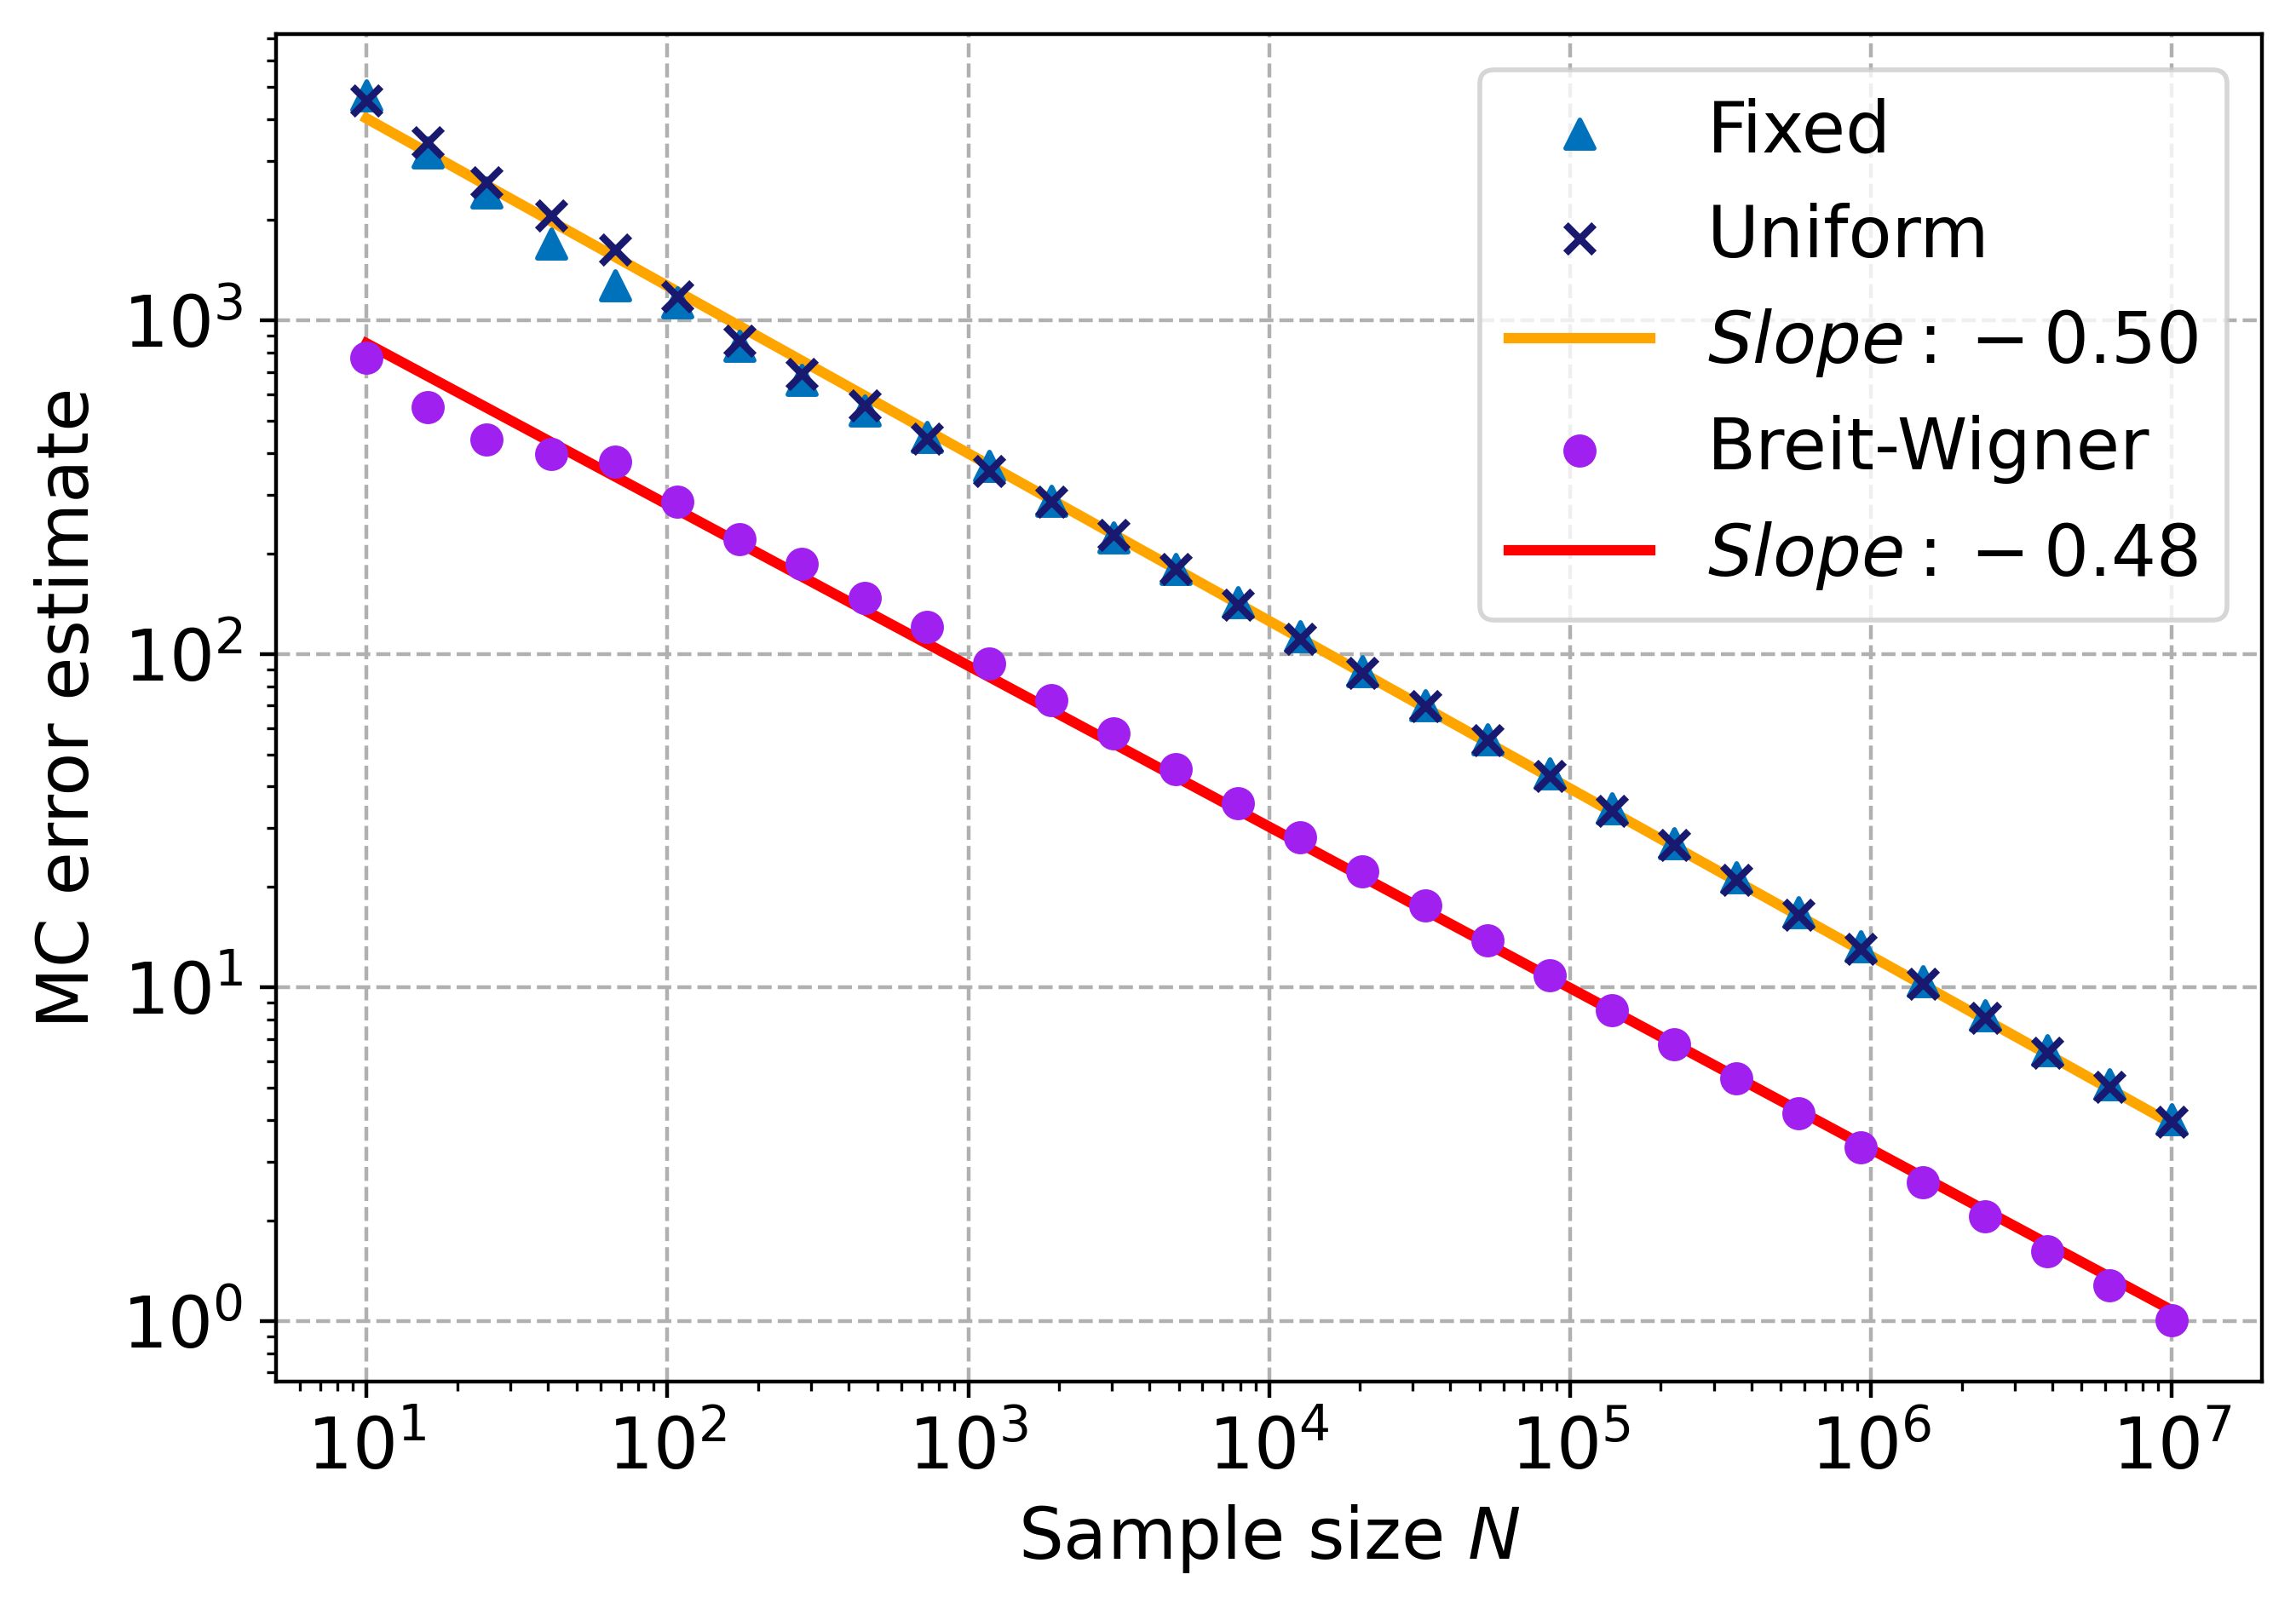
\includegraphics[width=\linewidth]{figures/ex1_all_mc_errors.png}
    \captionof{figure}{Monte Carlo error estimate of the cross-section vs. sample size for the three different cases of $s$ sampling.}
    \label{fig:1-mc-errors}
\end{minipage} \hfill
\begin{minipage}{0.47\linewidth}
    \centering
    \captionsetup{type=figure}
    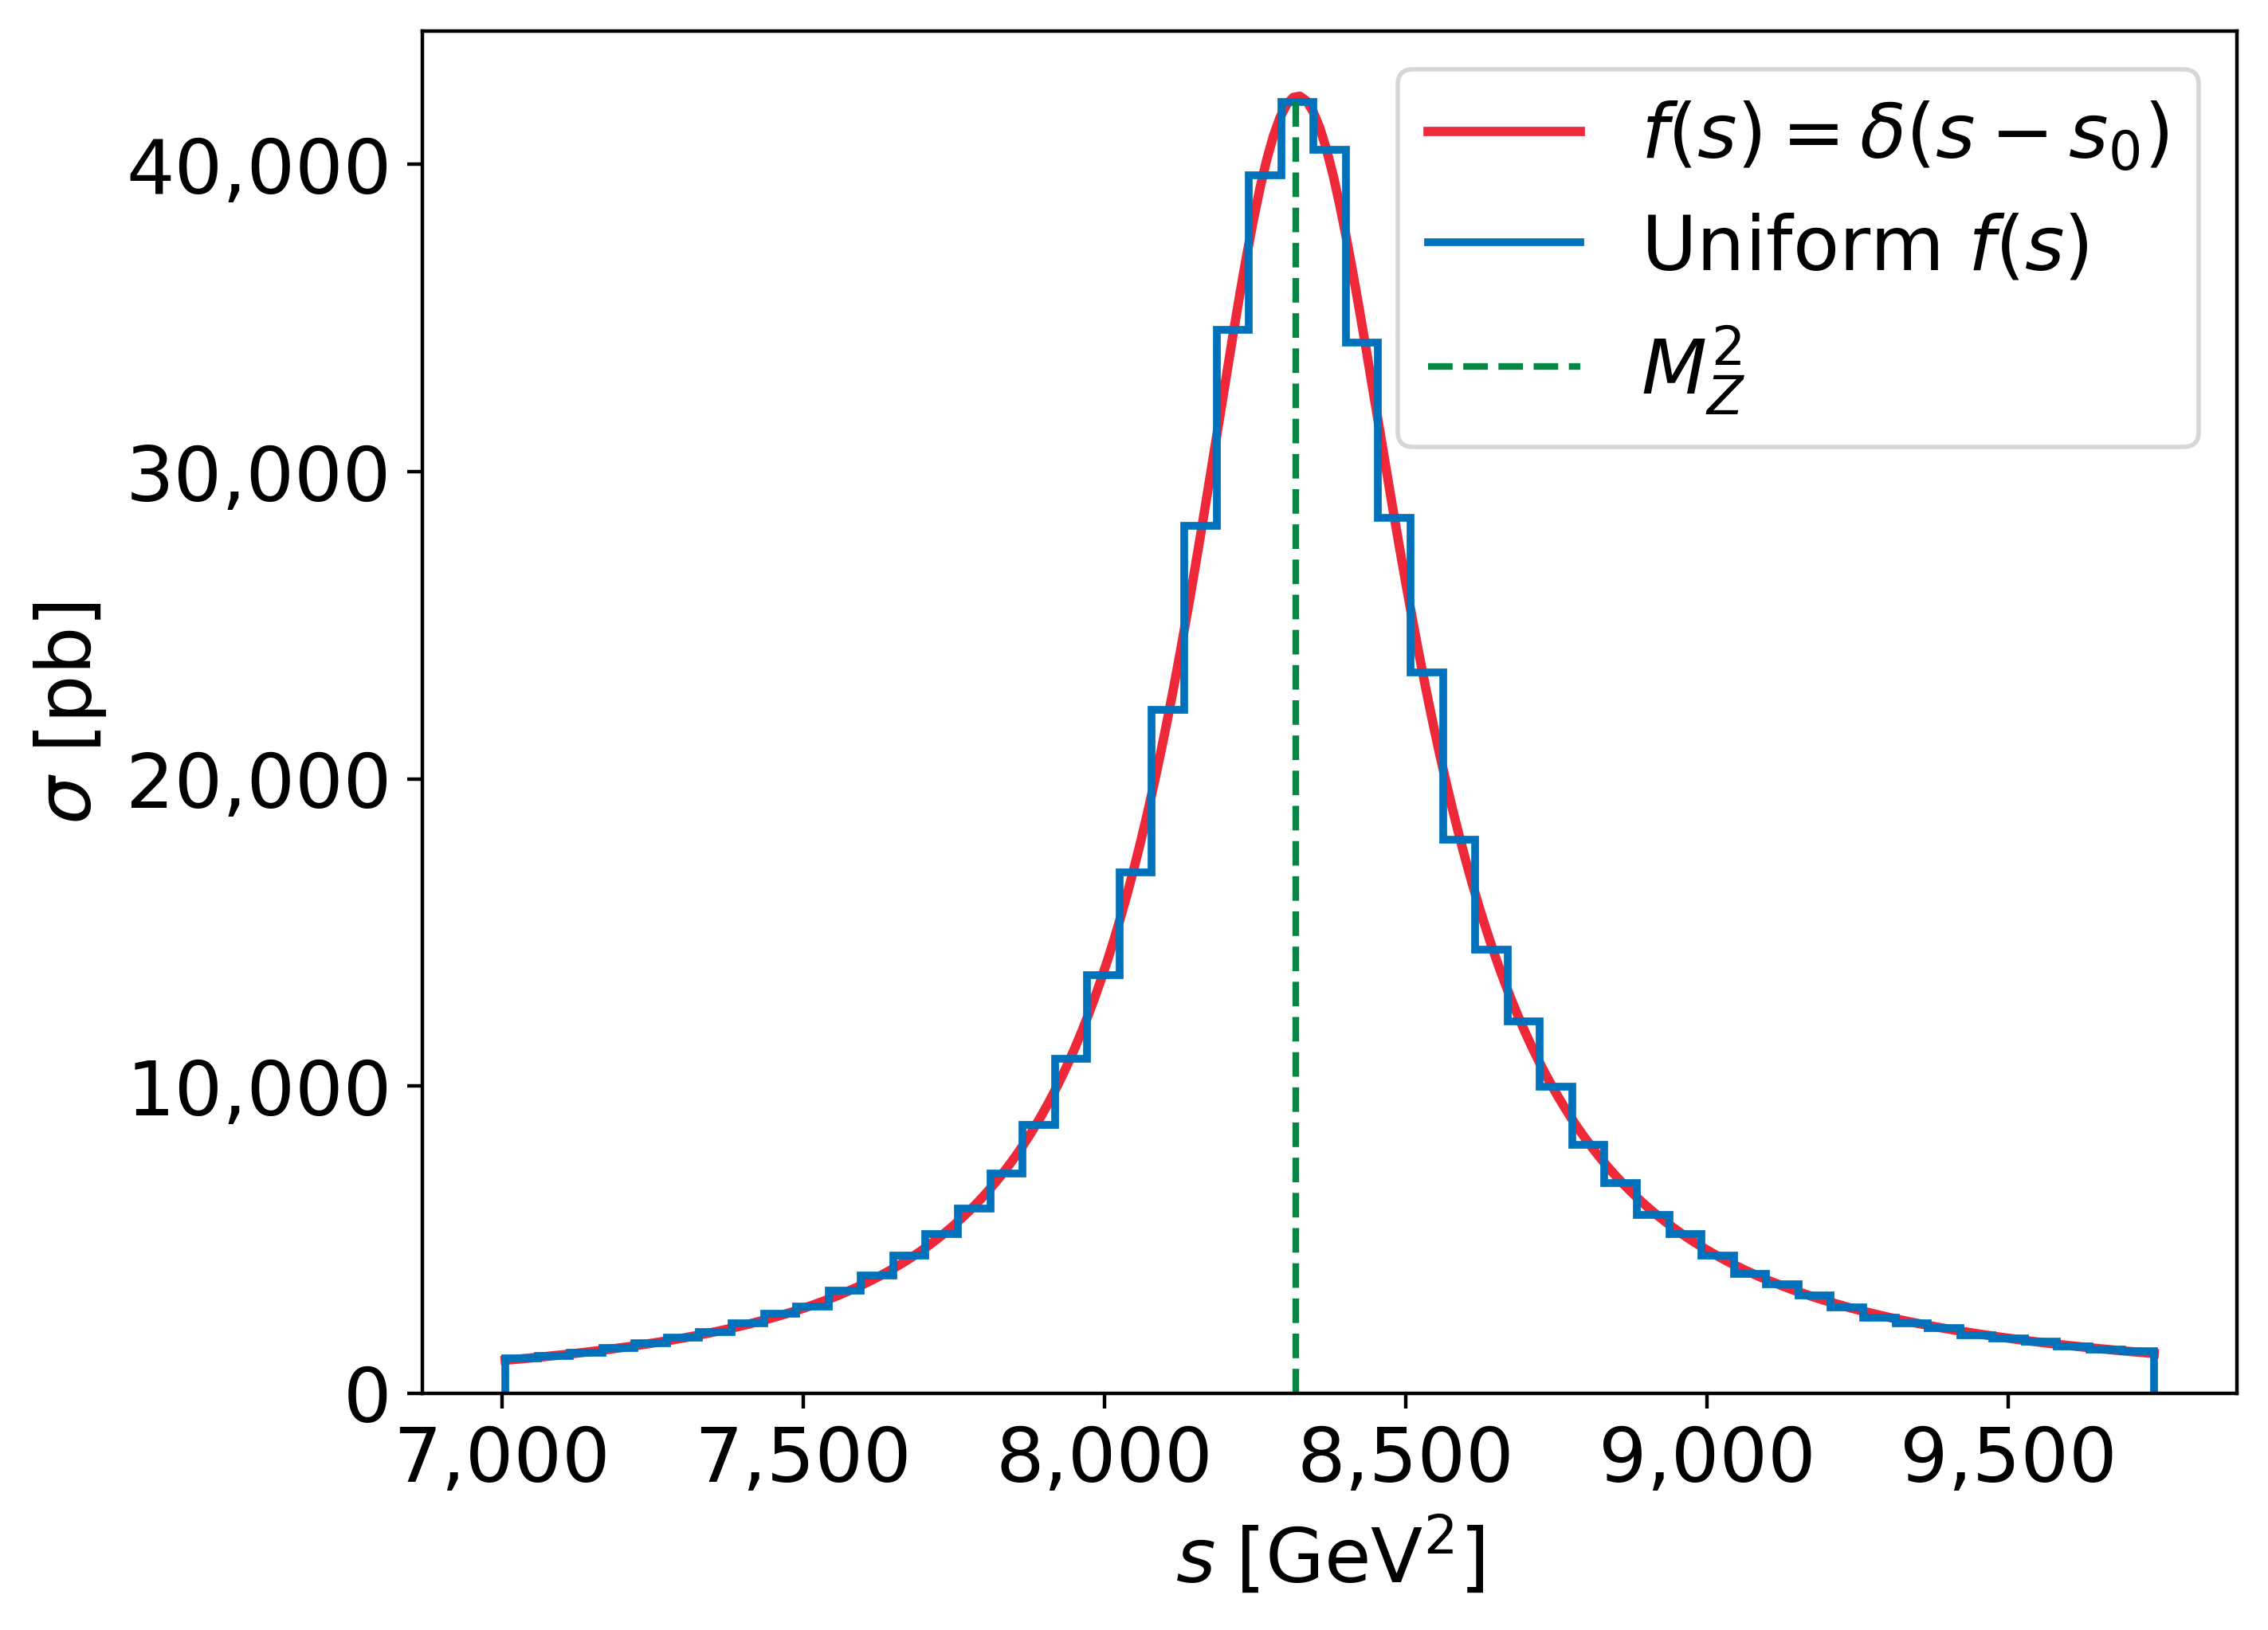
\includegraphics[width=\linewidth]{figures/ex1_part_d_histo.png}
    \captionof{figure}{Cross-section values from binning the flat beam spectrum vs. integration at fixed beam energy.}
    \label{fig:ex1d_histogram}
\end{minipage}

\medskip

The fact that the values of the cross-section are distributed along $s$ in the shape found in \autoref{fig:ex1d_histogram}, is precisely what motivates sampling $s$ according to the Breit-Wigner distribution with the Z boson as the resonance (well, that and the whole theoretical background, of course), equation \eqref{eq:1-breit-wigner}. This distribution has a global maximum at $M_{\mathrm{Z}}^{2}$, decaying to both sides, besides resembling the common factor present in both $\chi_{1}(s)$ and $\chi_{2}(s)$, equation \eqref{eq:1-chi-funcs}. Thus, the Breit-Wigner distribution seems to capture well the importance of different $s$ values to the integral for the cross-section, providing a more reasonable distribution for sampling $s$ rather than a uniform distribution. This is indeed the case, as can be seen from the Monte Carlo error estimates in \autoref{tab:1-cross-sections} and \autoref{fig:1-mc-errors}, where \marginpar{Part g)}\emph{the errors are four times smaller than the uniform case for the same sample size}.

\subsection{Vegas}

The improvement in accuracy of Monte Carlo methods when estimating integrals, as a result of using importance sampling with a distribution that captures enough features of the integrand, has led to develop sophisticated algorithms to determine such distributions. An example of these, is the implementation of Monte Carlo integration in the \texttt{vegas} package for python. This package implements the VEGAS algorithm, consisting on “scanning” over several passes the integration region and making a histogram that approximates the distribution of the integrand. In particular, the package implements two adaptive strategies: importance sampling and adaptive stratified sampling. Thus, an integration problem using the \texttt{vegas.Integrator}\textsuperscript{\texttrademark} is characterized solely by a region of integration and an integrand. After this, a number of evaluations \texttt{neval} (how many times to evaluate the integrand) and a number of iterations \texttt{nint} (number of times to perform \texttt{neval} evaluations of the integrand) yield independent estimations of the integral. A complete discussion of its implementation and use of the package can be found in \url{https://vegas.readthedocs.io/en/latest/tutorial.html}. 

Using 10 iterations with 1,000 Monte Carlo points each, the differential cross-section in equation \eqref{eq:1-diff-sigma} was integrated with \texttt{vegas}, obtaining the results shown in \autoref{tab:1-vegas-summary}. Here, the first two iterations are not to be taken into account, shown by the relatively high values of $Q$ (the $p$-value of the $\chi^{2}$) as compared with the rest of the subsequent iterations. This is because during these iterations vegas has not yet been able to fully optimize the sampling for the integrand. However, for every iteration after the second, the error decreases consistently, reaching a weighted average result of 9,930 pb with an error estimate of 14 pb, only 1pb of difference from the exact value of 9,929 pb.

\begin{table}[ht!]
    \centering
    \renewcommand{\arraystretch}{1.2}
    \begin{tabular}{rcccc}
    \hline Iteration & Integral & Weighted average & $\chi^{2} /$ d.o.f. & $Q$ \\ \hline
    1 & 9,720(17) & 9,720(17) & 0.00 & 1.00 \\
    2 & 10,030(10) & 9,948(87) & 2.54 & 0.11 \\
    3 & 9,653(79) & 9,787(59) & 4.42 & 0.01 \\
    4 & 9,952(70) & 9,855(45) & 4.05 & 0.01 \\
    5 & 9,933(54) & 9,887(35) & 3.34 & 0.01 \\
    6 & 9,933(52) & 9,901(29) & 2.79 & 0.02 \\
    7 & 9,878(42) & 9,894(24) & 2.35 & 0.03 \\
    8 & 9,899(38) & 9,895(20) & 2.02 & 0.05 \\
    9 & 9950(33) & 9,910(17) & 2.01 & 0.04 \\
    10 & 9,977(26) & 9,930(14) & 2.29 & 0.01 \\ \hline
    \end{tabular}
    \caption{Summary of the vegas integration for 10 iterations of 1,000 Monte Carlo points each. The “Integral” and “Weighted average” columns correspond to estimations for the cross-section in picobarns. $Q$ represents the $p$-value of the $\chi^{2}$.}
    \label{tab:1-vegas-summary}
\end{table}

The remarkably good estimation for the cross-section with relatively few evaluations is made possible due to the fact that \texttt{vegas} has been able to “flatten” the integral, i.e., find a transformation of the integration variables such that their sampling captures better the integrand. This can be seen in \autoref{fig:ex1e_one_grid}, which shows the optimal integration grid found by vegas for the variables $s$ and $\cos{\theta}$ (since there is no dependence on $\phi$). The other two integration grids, for the pairs $(s, \phi)$ and $(\cos{\theta}, \phi)$, are shown in \autoref{sec:app-int-grids}. Although the accumulation of $s$ values close to $M_{\text{Z}}^{2}$ was to be expected, \marginpar{Part e)} \emph{smaller binning for values of $\cos{\theta}$ close to +1 and -1 come as a surprise}. Indeed, this is made clear by plotting the integrand, as shown in \autoref{fig:ex1e-integrand-plot}, where peaks towards these values can be seen, and the peak at +1 is larger than that at $-1$.

\begin{figure}[ht!]
    \centering
    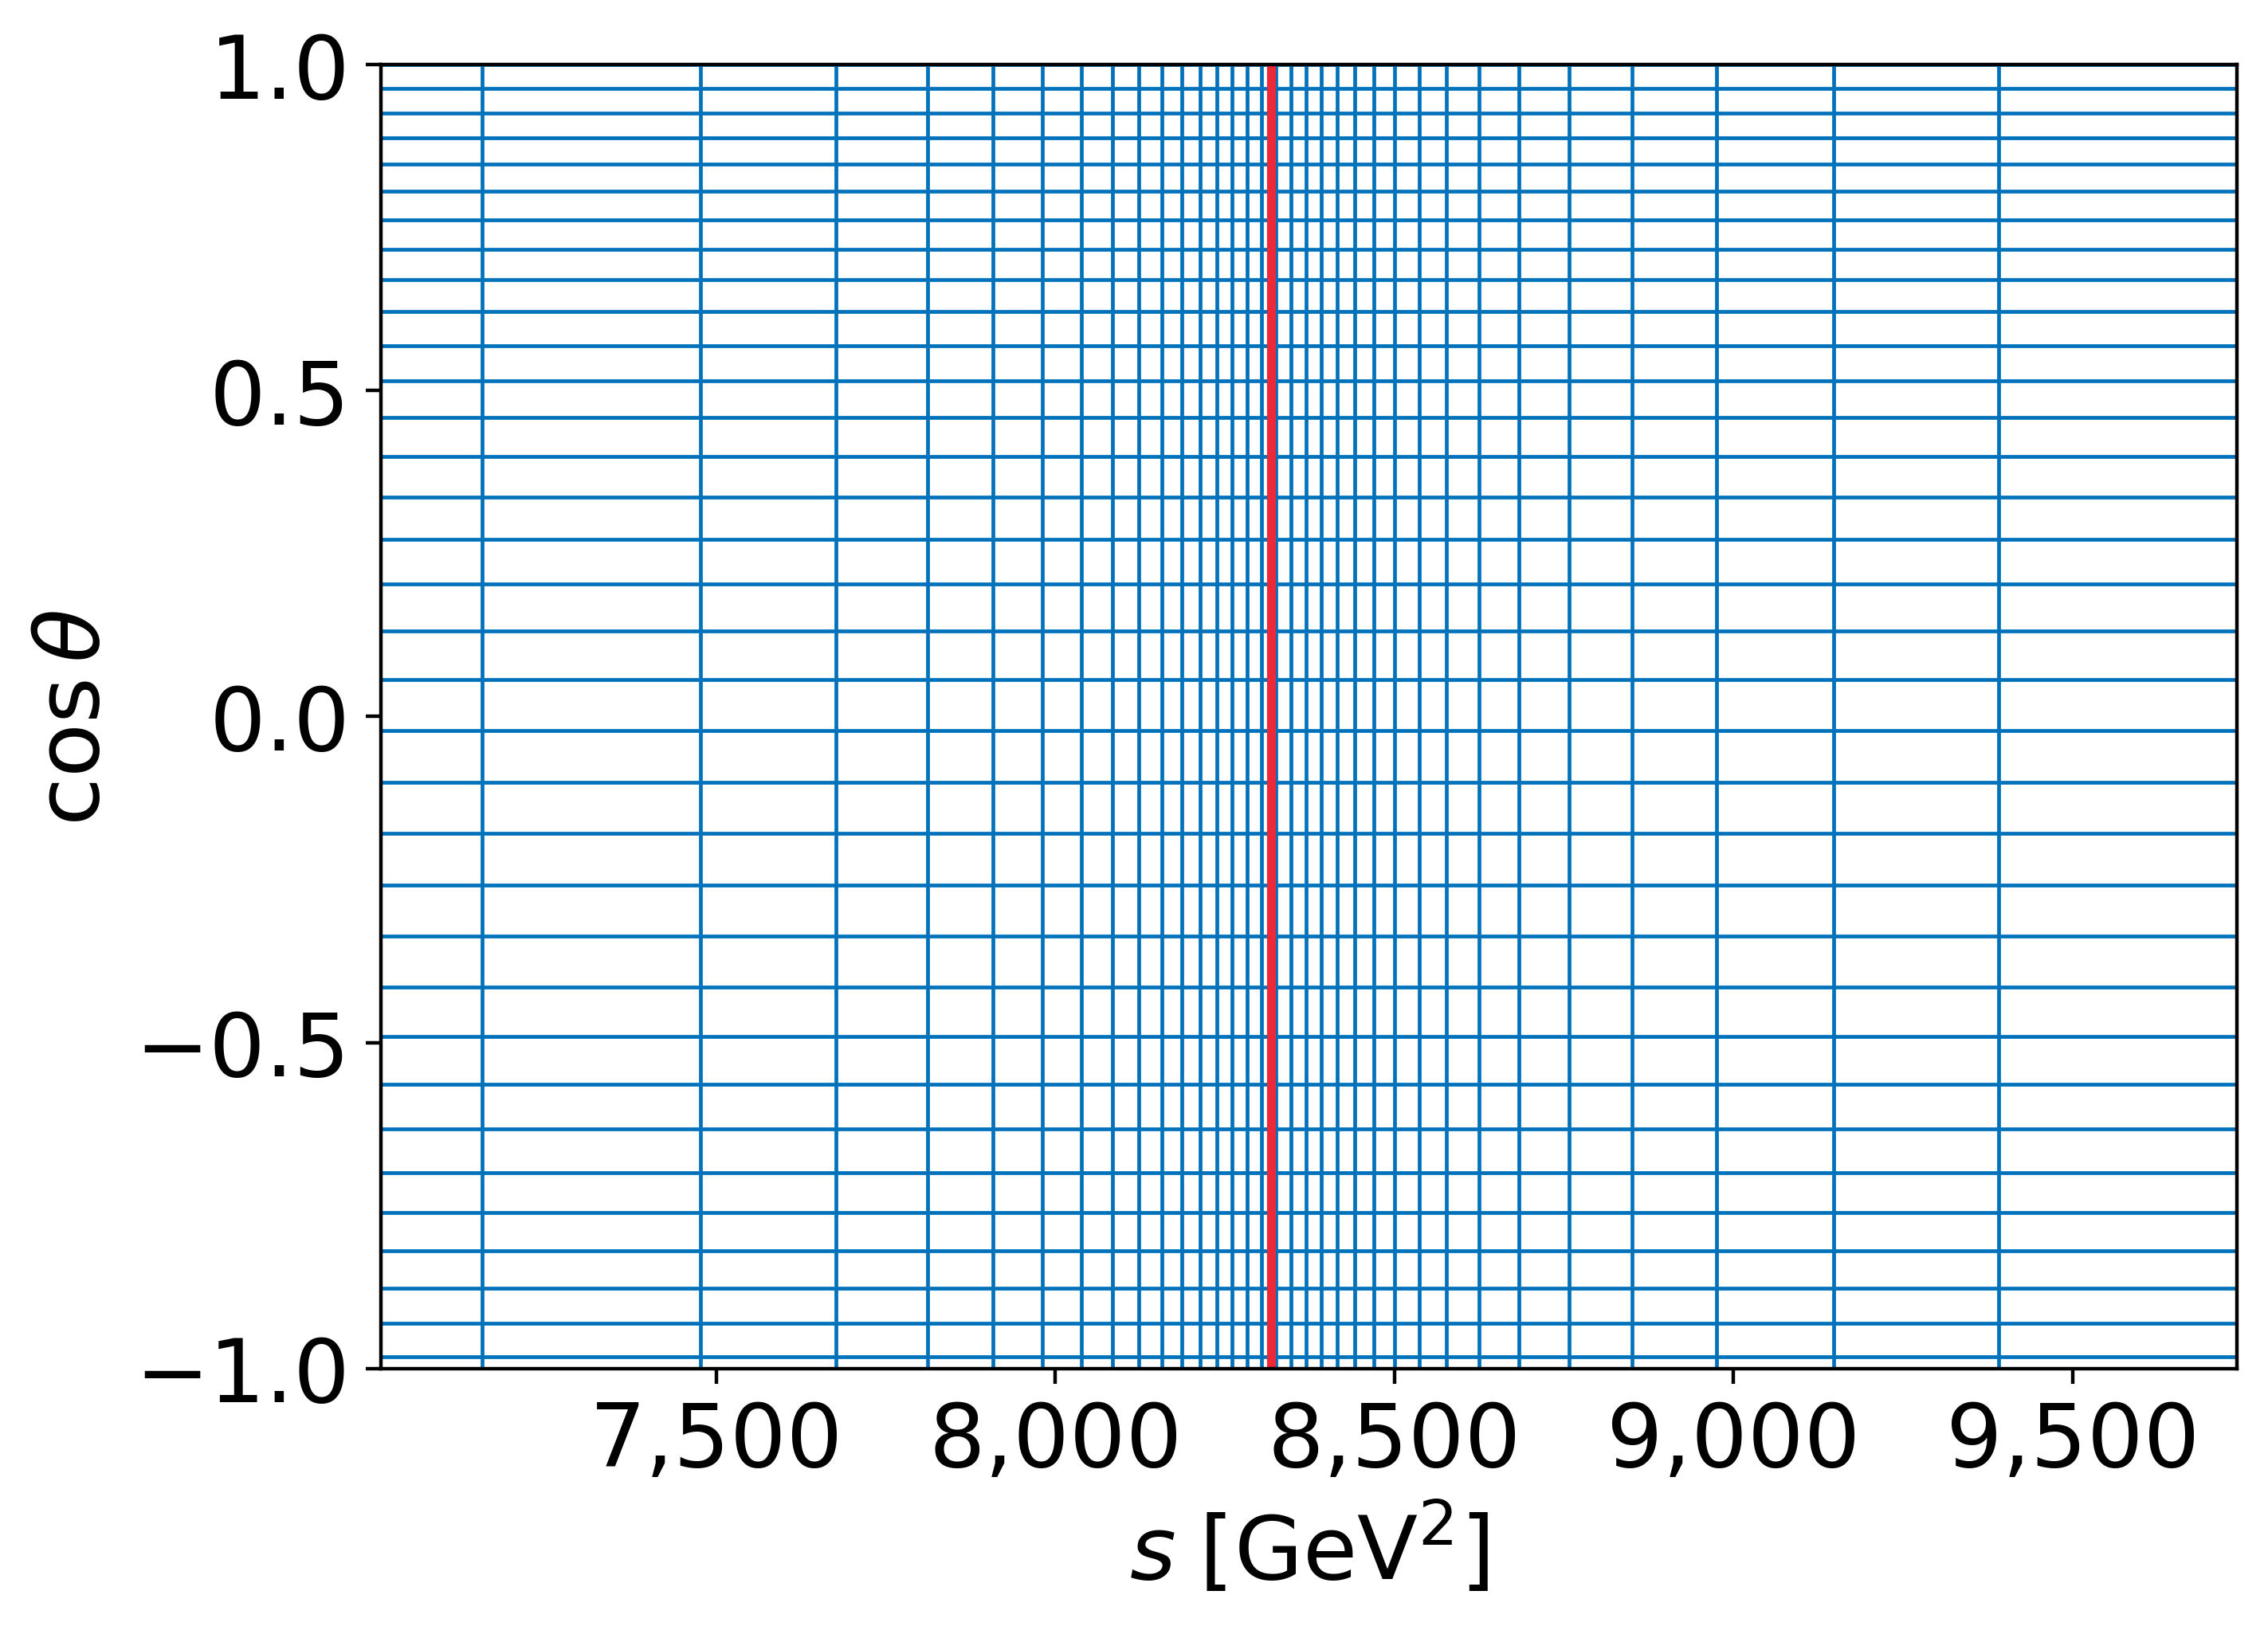
\includegraphics[width=0.6\linewidth]{figures/integration_grid_0.png}
    \caption{Binning of the integration grid found by \texttt{vegas} after 10 iterations of 1,000 evaluations each.}
    \label{fig:ex1e_one_grid}
\end{figure}

\begin{figure}
    \centering
    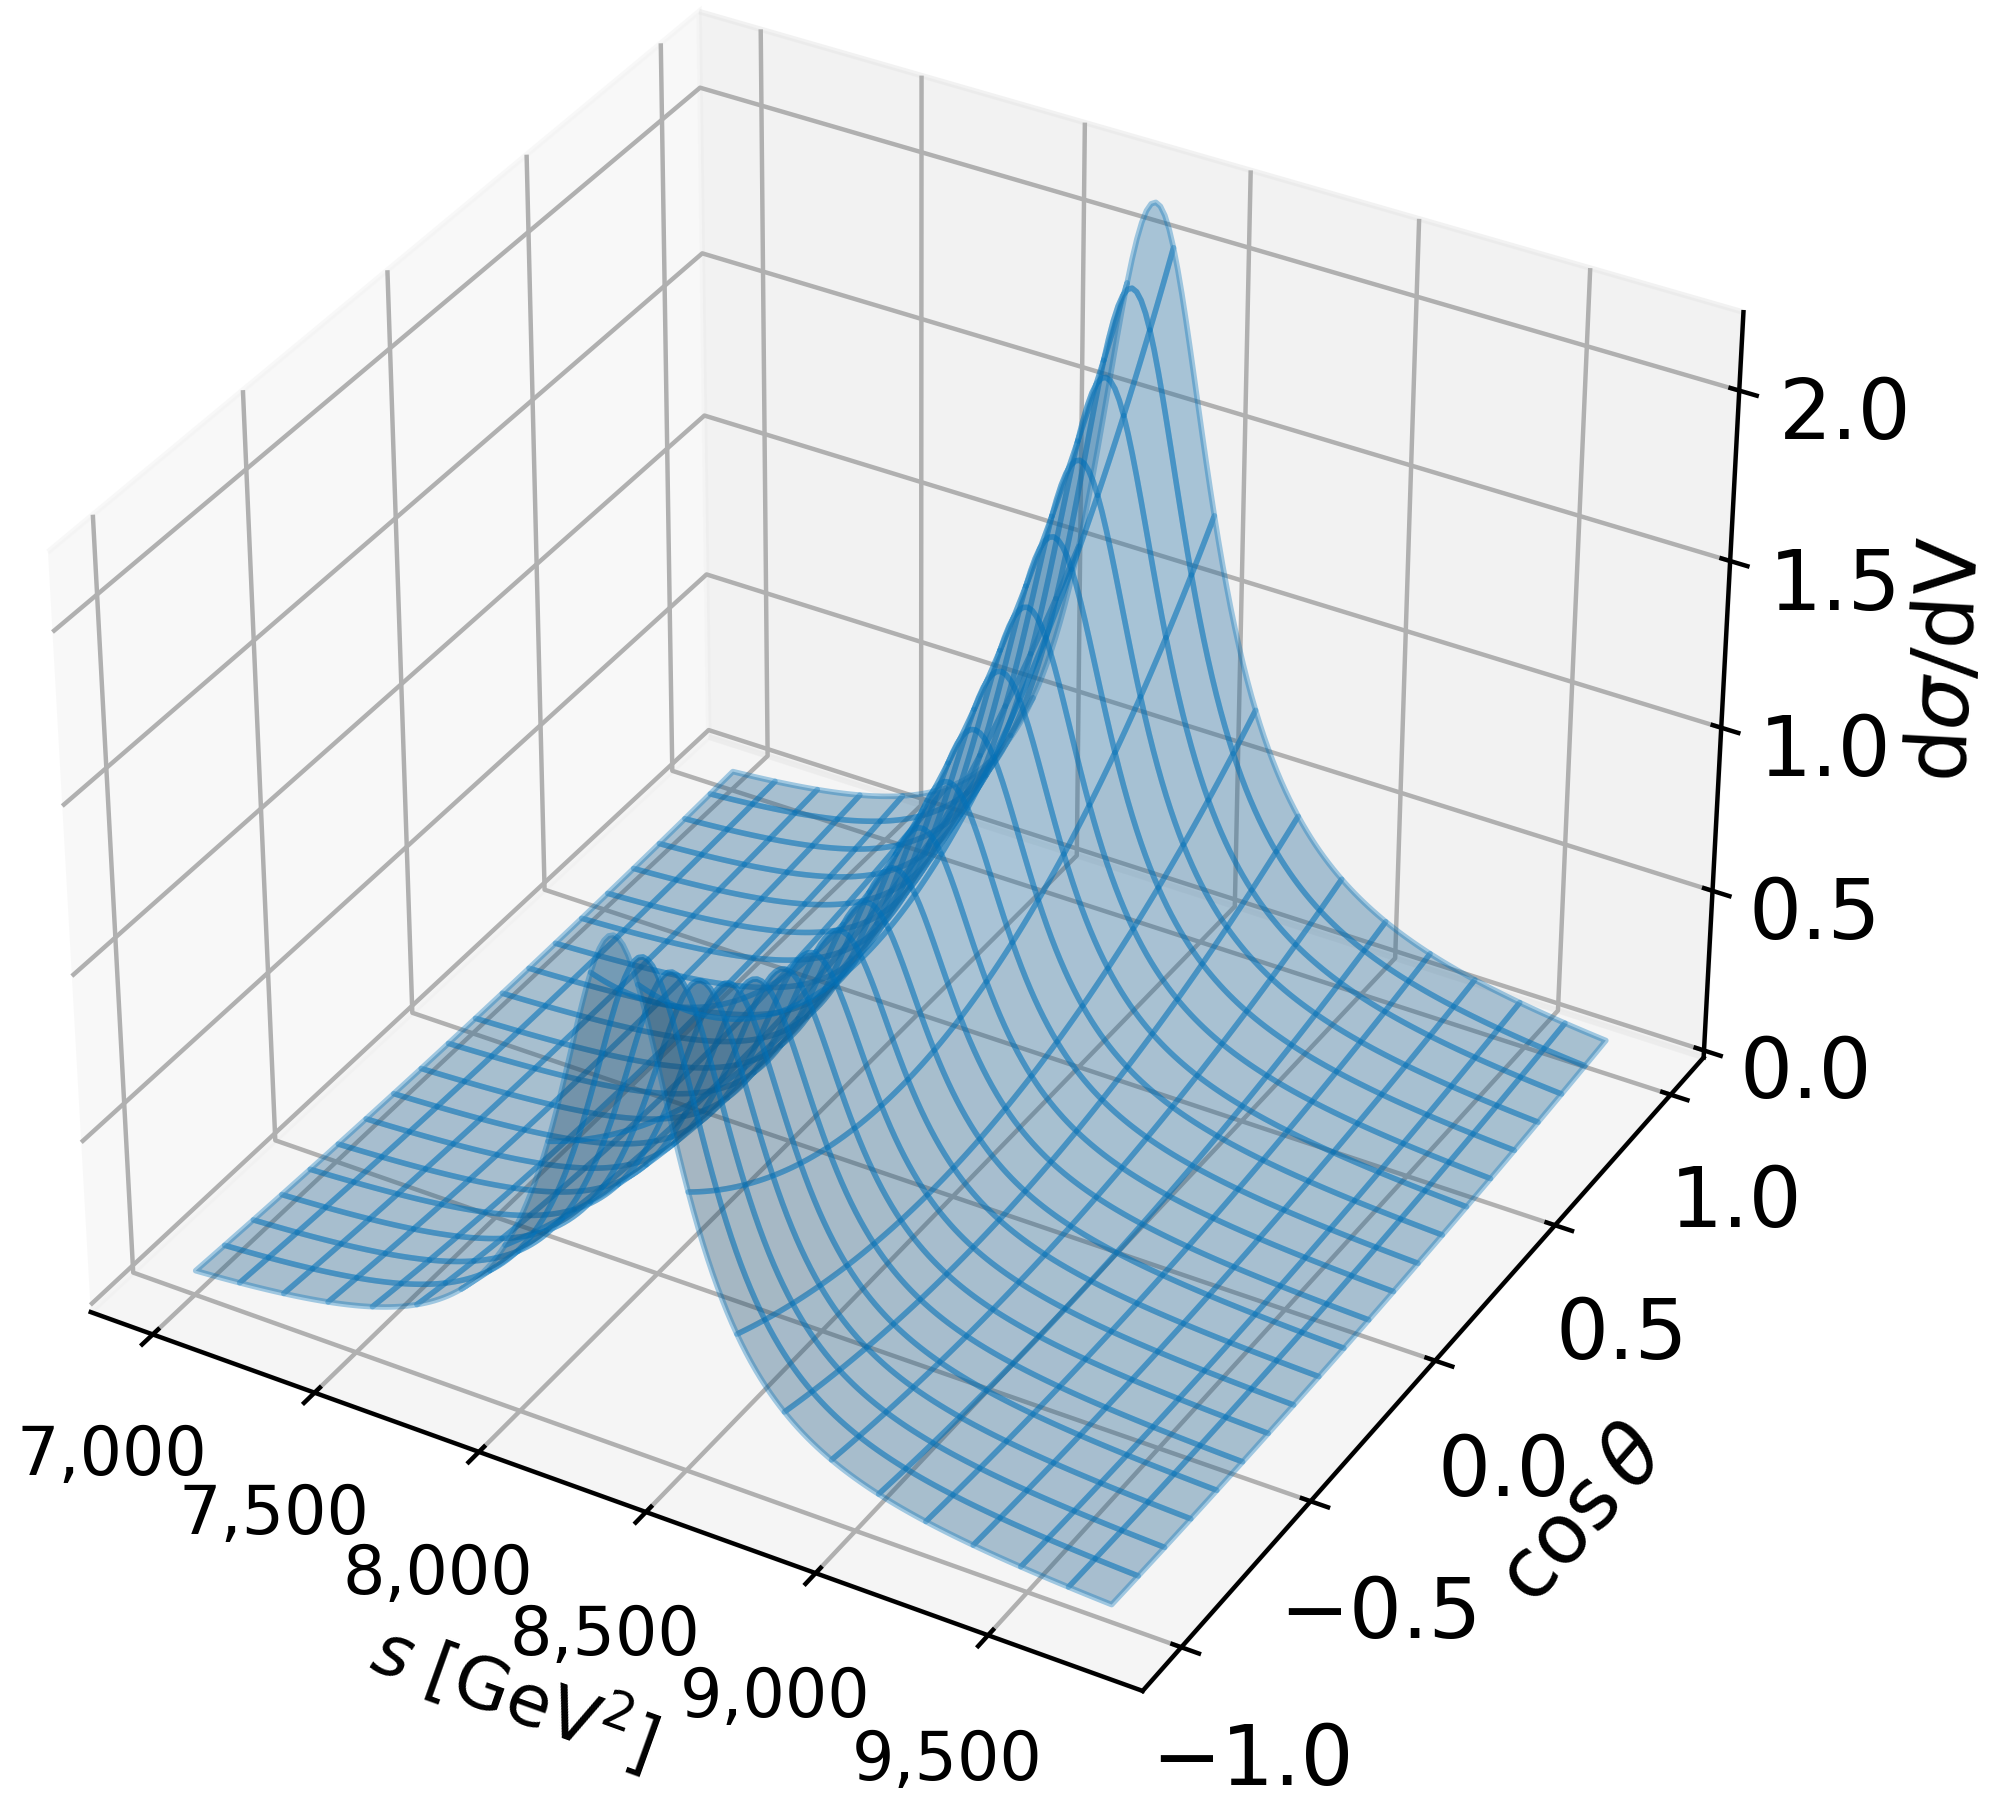
\includegraphics[width=0.6\linewidth]{figures/integrand_plot.png}
    \caption{Differential cross-section per volume. Here $\mathrm{d}V = \mathrm{d}s \, \mathrm{d}(\cos{\theta}) \mathrm{d}\phi$.}
    \label{fig:ex1e-integrand-plot}
\end{figure}

% \begin{minipage}{0.47\linewidth}
%     \centering
%     \captionsetup{type=figure}
%     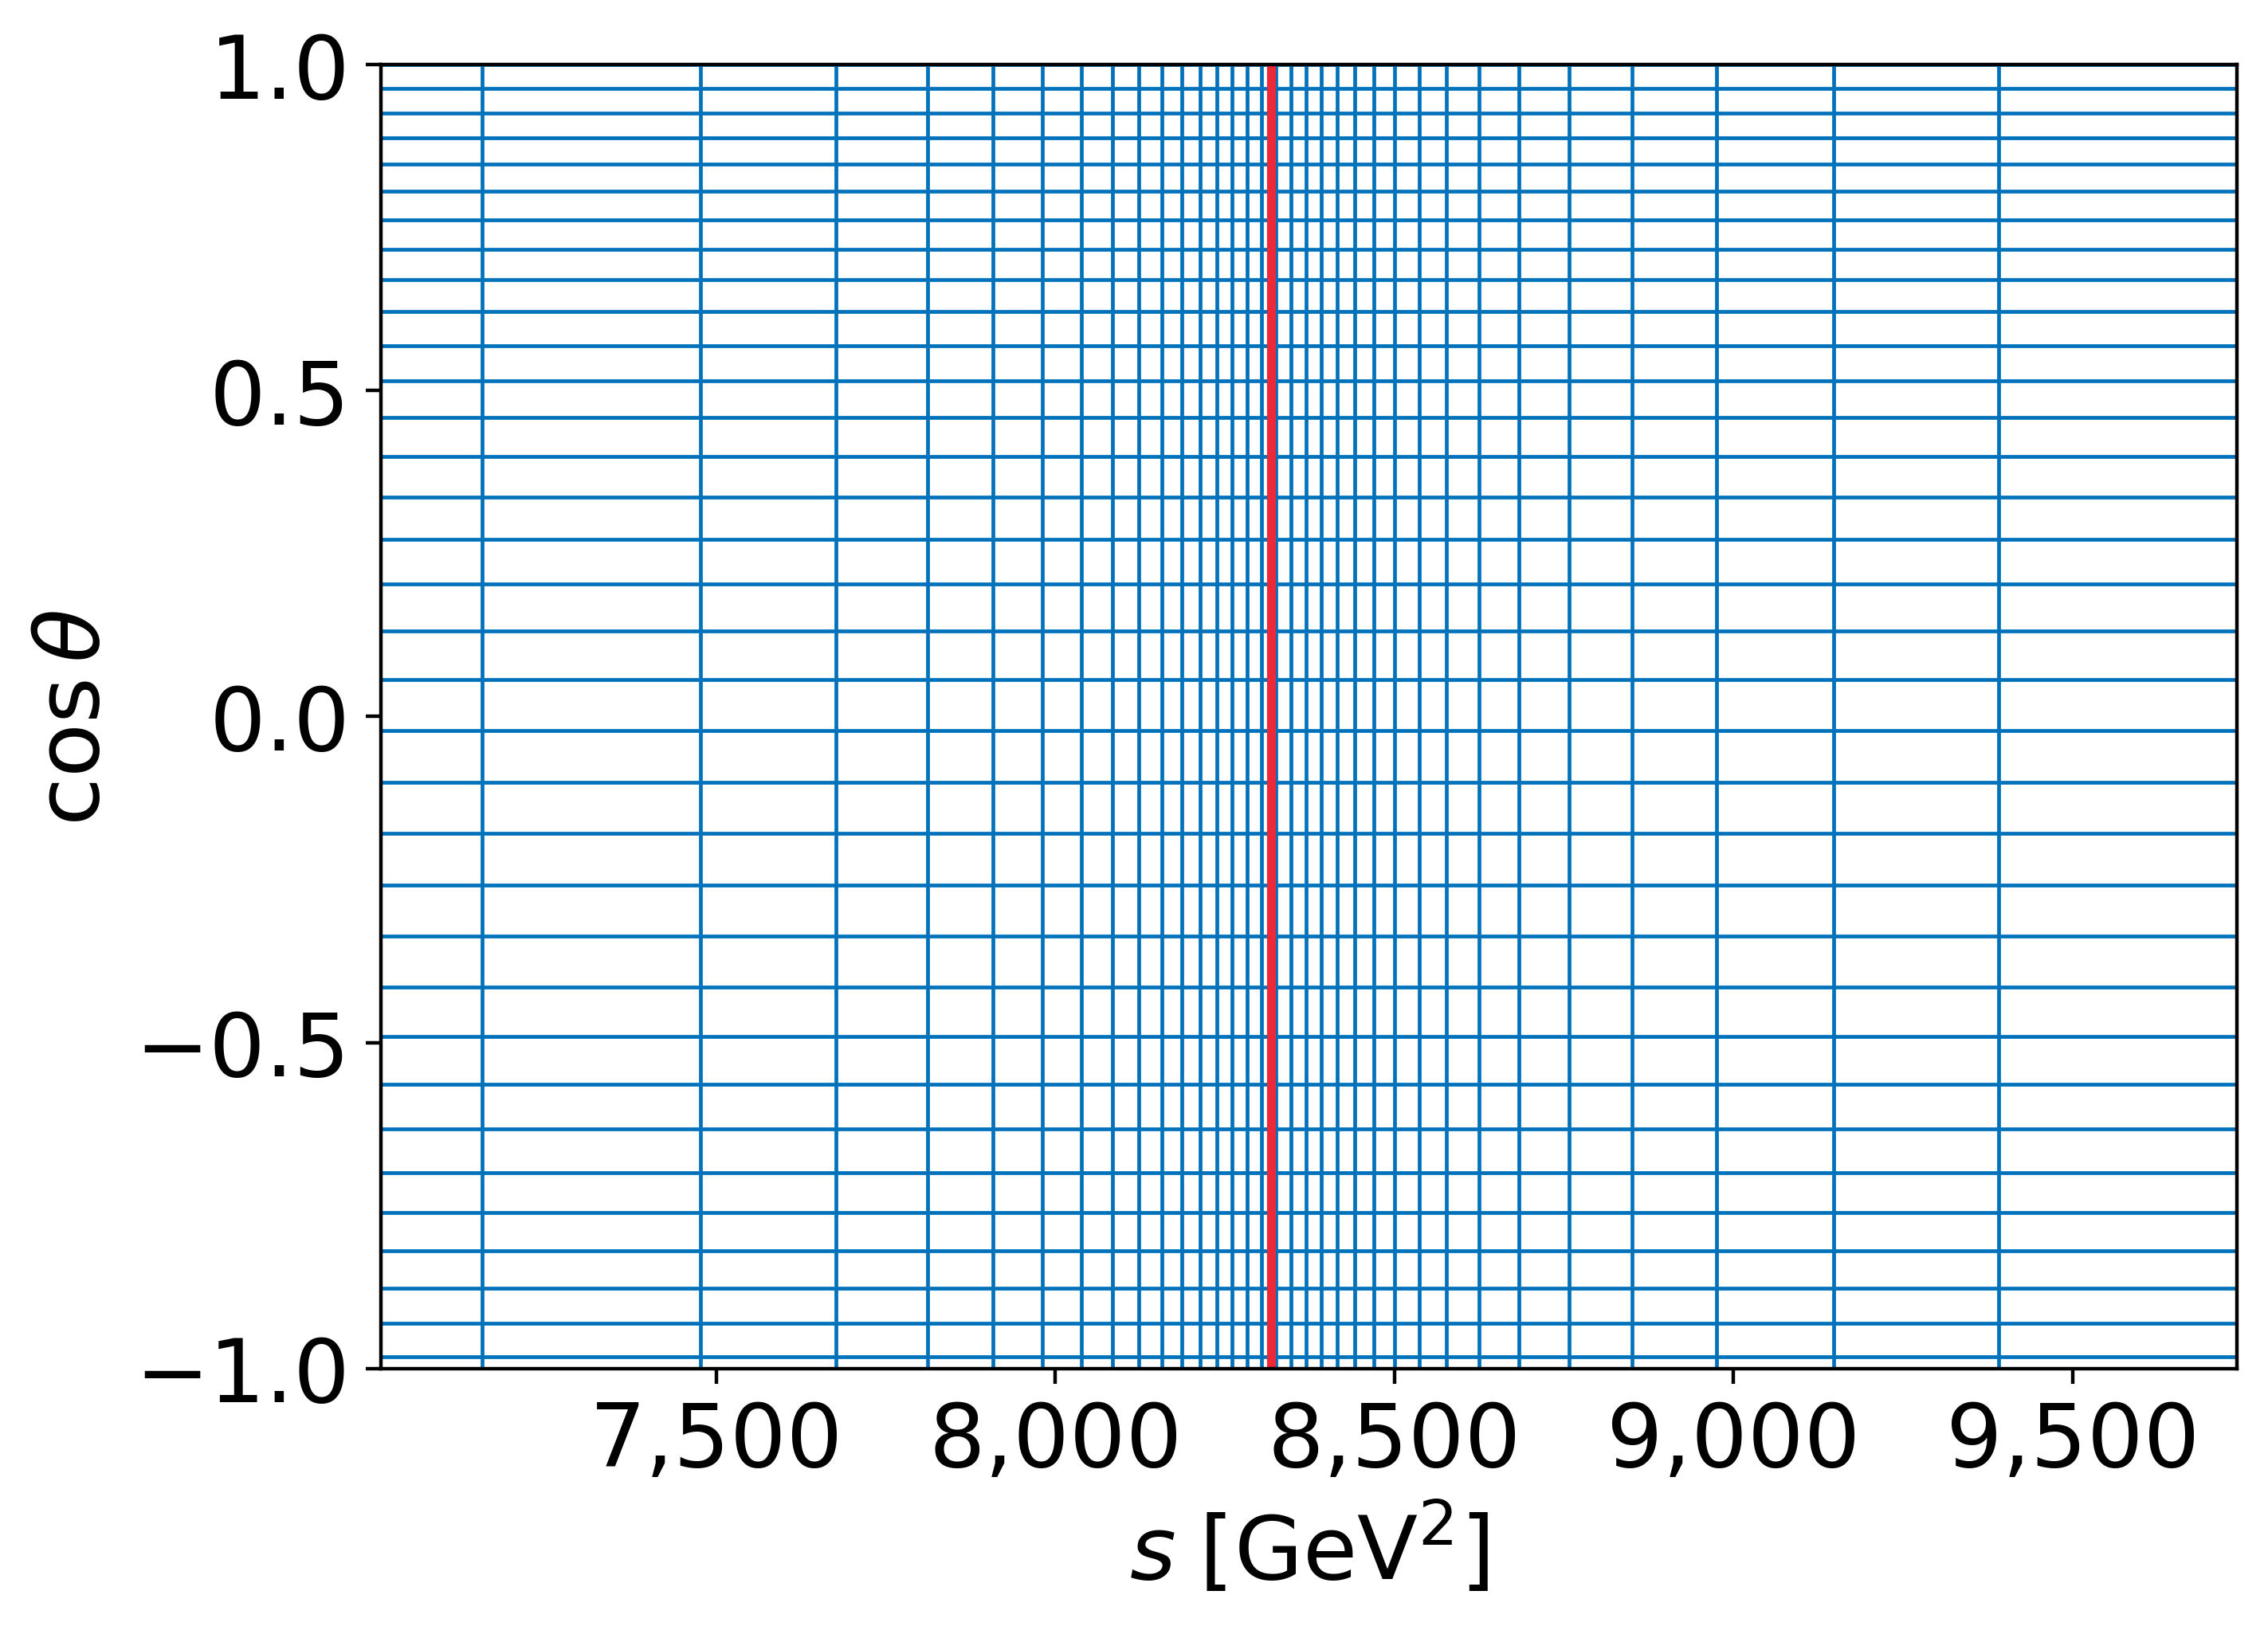
\includegraphics[width=\linewidth]{figures/integration_grid_0.png}
%     \caption{Binning of the integration grid found by \texttt{vegas} after 10 iterations of 1,000 evaluations each.}
%     \label{fig:ex1e_one_grid}
% \end{minipage} \hfill
% \begin{minipage}{0.47\linewidth}
%     \centering
%     \captionsetup{type=figure}
%     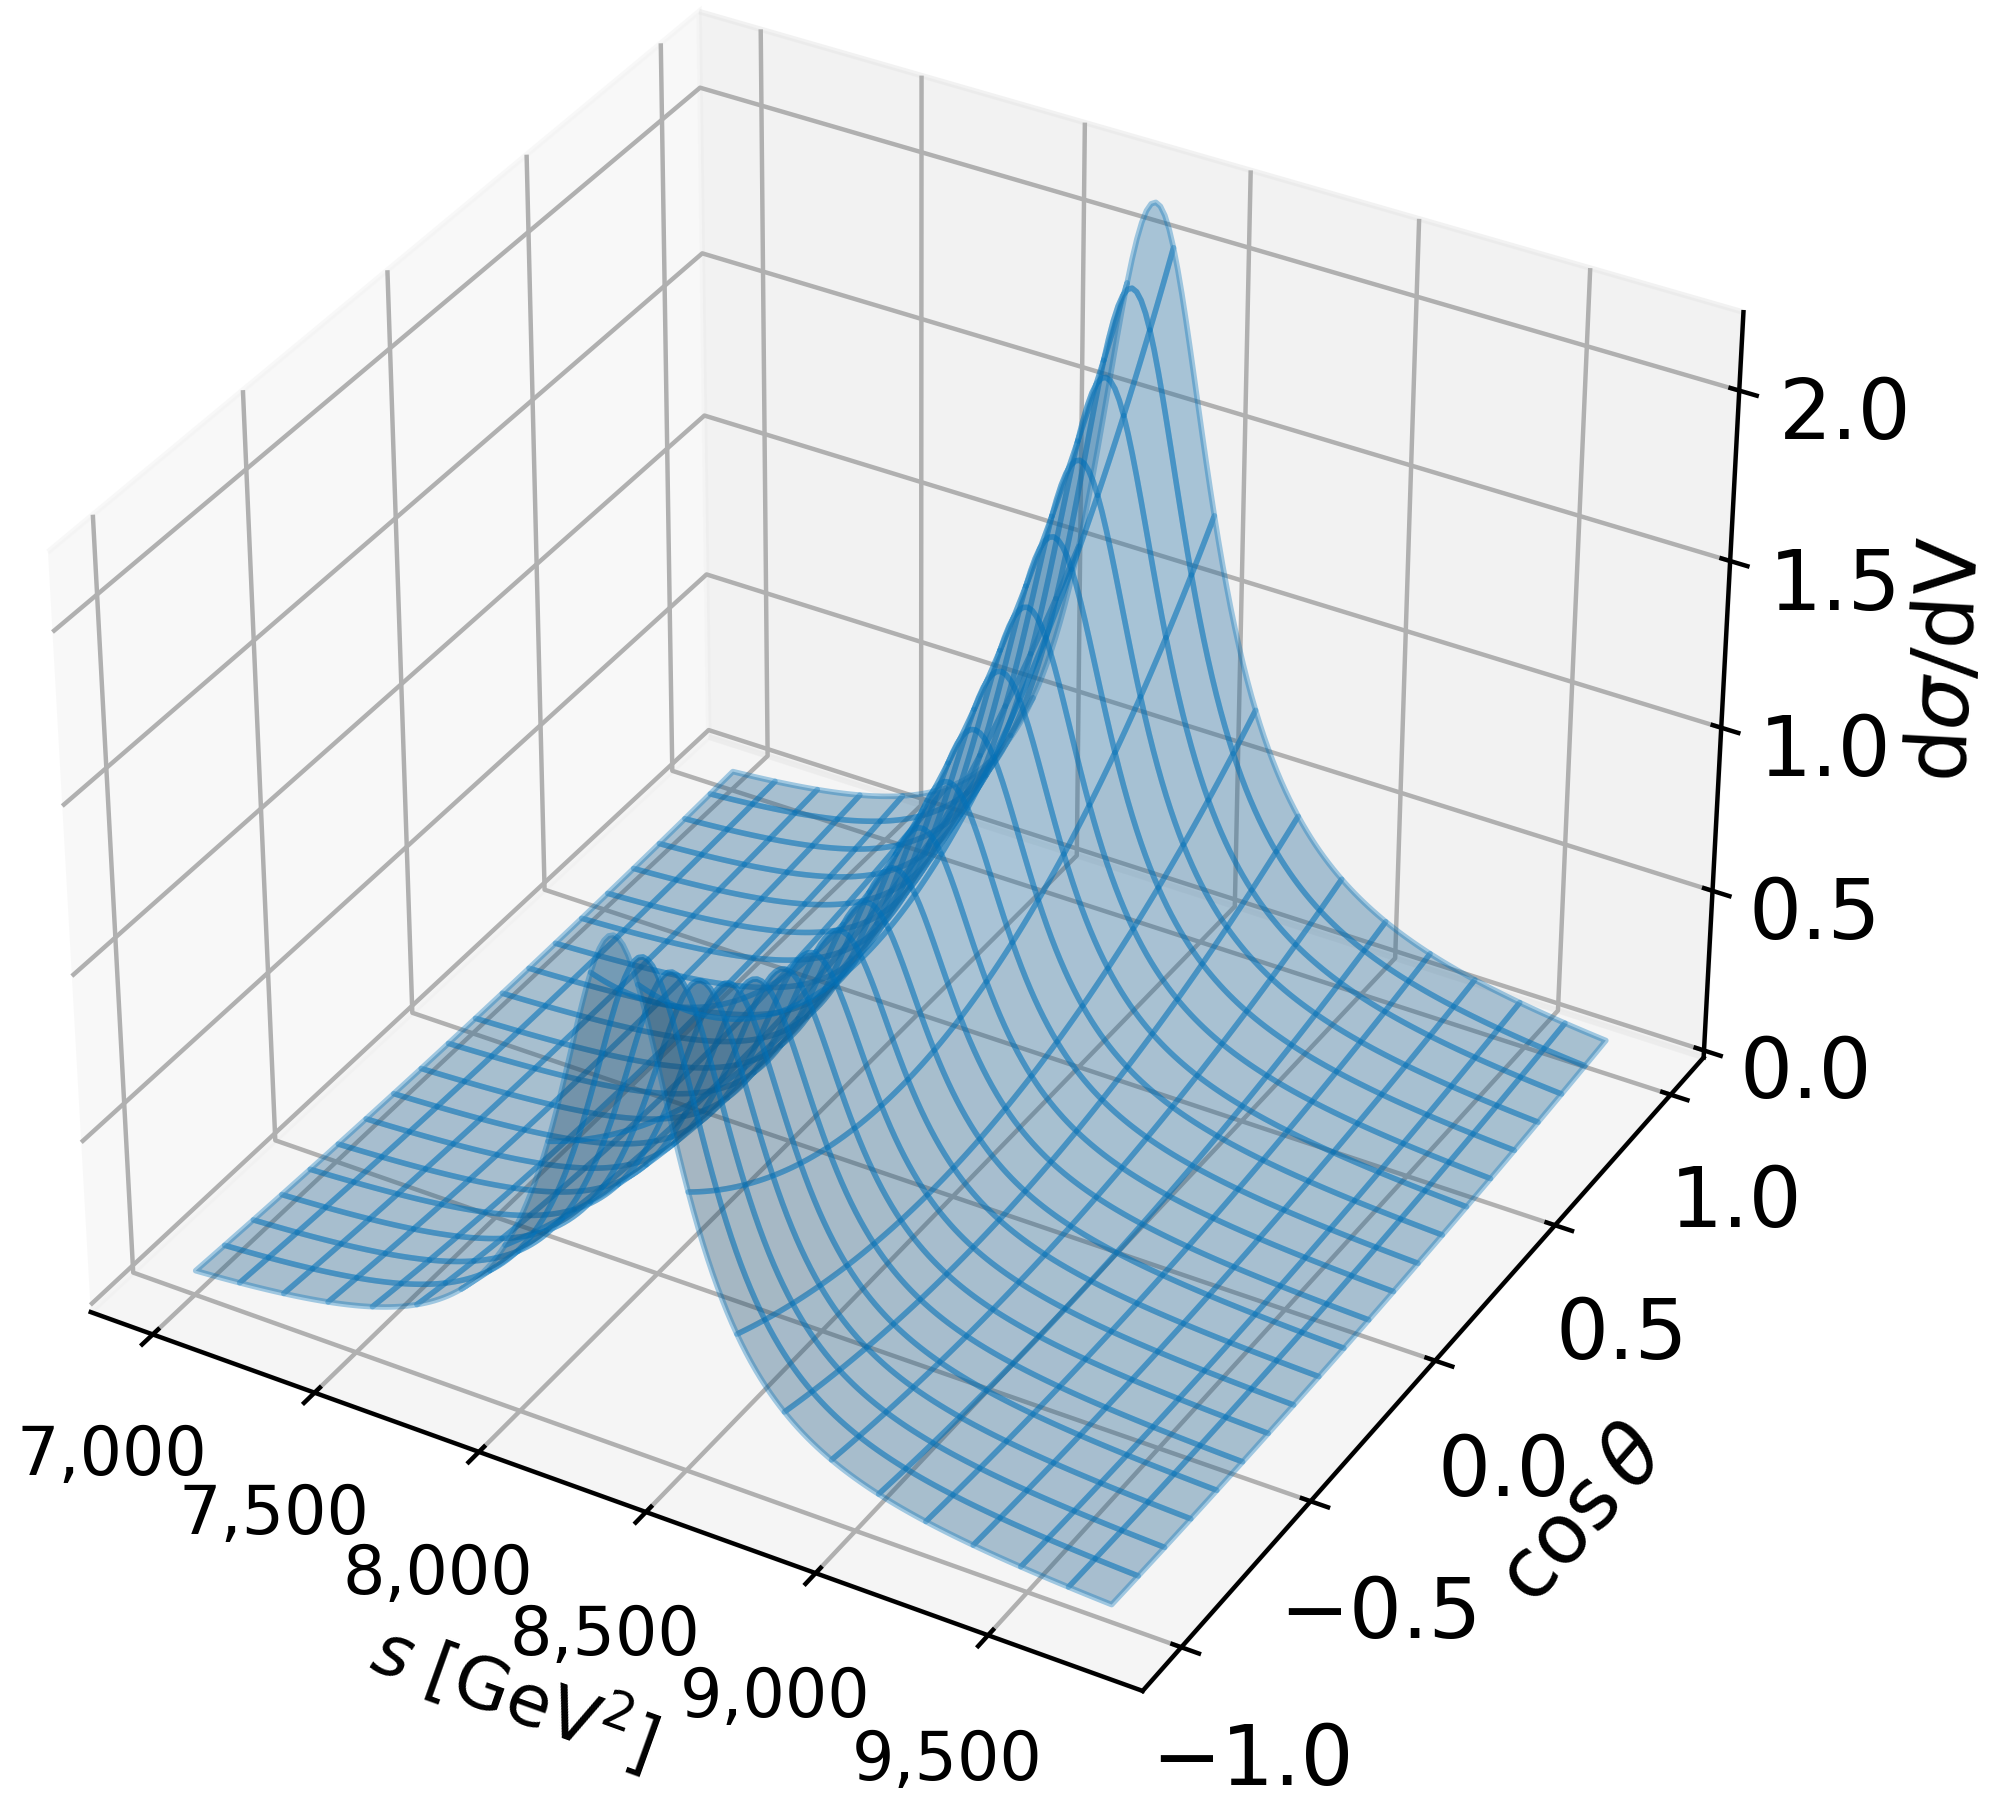
\includegraphics[width=\linewidth]{figures/integrand_plot.png}
%     \captionof{figure}{Differential cross-section per volume. Here $\mathrm{d}V = \mathrm{d}s \, \mathrm{d}(\cos{\theta}) \mathrm{d}\phi$.}
%     \label{fig:ex1e-integrand-plot}
% \end{minipage}
